\chapter{Fungsi dan Prosedur}

\section{Petunjuk}
\begin{itemize}
	\item Perhatikan petunjuk Dosen untuk berbagai permasalahan Fungsi dan Prosedur  !
	\
	\item Perhatikan dan ikuti petunjuk dosen mengenai bagaimana cara menggunakan program Judge untuk mengevaluasi permasalahan yang Anda kerjakan!
\end{itemize}

\pagebreak
\section{Permasalahan}
\begin{permasalahan}{Berapa Kata ?}\\
\label{prob:BerapaKata}
	Diberikan sebuah kalimat dapatkah Anda menentukan ada berapa kata dalam kalimat tersebut ? \\\\
	\textbf{Masukan}\\
	Tipe data String yang berupa kalimat\\
	\textbf{Keluaran}\\
	Tipe data integer yang mewakili berapa kata dalam kalimat tersebut
	\begin{center}
	\textbf{Test Case}\\
	\end{center}
	\textbf{Masukan}\\
	Ibu Budi Pergi Ke Pasar\\
	\textbf{Keluaran}\\
	5
	\\\\
	
	Anda diminta untuk membuat sebuah fungsi untuk penyelesaian masalah ini dengan ketentuan : \\
	\begin{itemize}
		\item \textit{hitungKata(String) : integer}\\
	\end{itemize}
\end{permasalahan}


\newpage

\begin{permasalahan}{Diatas Rerata !}\\
\label{prob:DiatasRerata}
	Diberikan kumpulan nilai dari seluruh mahasiswa dari sebuah kelas dapatkah Anda menentukan berapa persen
		mahasiswa yang dikategorikan diatas rata - rata ? \\\\
	\textbf{Masukan}\\
	Kumpulan bilangan bulat yang mewakili nilai - nilai mahasiswa \\
	\textbf{Keluaran}\\
	Pecahan yang mewakili persentase mahasiswa diatas rata - rata
	\begin{center}
	\textbf{Test Case 1}\\
	\end{center}
	\textbf{Masukan}\\
	100 99 98 97 96 95 94 93 91\\
	\textbf{Keluaran}\\
	55.556\%
	
	\begin{center}
	\textbf{Test Case 2}\\
	\end{center}
	\textbf{Masukan}\\
	70 90 80\\
	\textbf{Keluaran}\\
	33.333\%

	\begin{center}
	\textbf{Test Case 3}\\
	\end{center}
	\textbf{Masukan}\\
	70 90 81\\
	\textbf{Keluaran}\\
	66.667\% 	 \\\\

	
	Anda diminta untuk membuat sebuah fungsi untuk penyelesaian masalah ini dengan ketentuan : \\
	\begin{itemize}
		\item \textit{diatasRerata(String) : float}\\\\
	\end{itemize}
	
	
	\textbf{Perhatian : Anda diharapkan mengembalikan bilangan pecahan dalam bentuk paling dasar tanpa formating dan tanpa simbol ``\%``, keluaran dengan format tiga dibelakang koma dan adanya persen adalah karena adanya pemanggilan pada MAIN PROGRAM}
	
	%credits : 20102113701
	
\end{permasalahan}

\begin{permasalahan}{Anagram}\\
\label{prob:anagram}
	Anagram adalah kata atau kalimat yang dibentuk dengan cara merubah susunan huruf dari kata atau kalimat lain. Dapatkah Anda menentukan bahwa sebuah kata adalah anagram dari kata lainnya ? \\\\
	\textbf{Masukan}\\
	Dua buah tipe data String\\
	\textbf{Keluaran}\\
	pernyataan ``anagram`` atau ``bukan anagram``\\
	\begin{center}
	\textbf{Test Case 1}\\
	\end{center}
	\textbf{Masukan}\\
	collation\\
	location\\
	\textbf{Keluaran}\\
	bukan anagram
	
	\begin{center}
	\textbf{Test Case 2}\\
	\end{center}
	\textbf{Masukan}\\
	Mother-In-Law\\
	Woman Hitler\\
	\textbf{Keluaran}\\
	anagram

	\begin{center}
	\textbf{Test Case 3}\\
	\end{center}
	\textbf{Masukan}\\
	I think therefore I am\\
  I fear to think I'm here\\
	\textbf{Keluaran}\\
	anagram\\\\

		\textbf{Perhatian : Pada test case INPUT akan terdapat simbol, spasi, dan huruf besar/kecil yang harus mampu Anda abaikan dalam pembuatan fungsi !} \\\\
	
	Anda diminta untuk membuat sebuah fungsi untuk penyelesaian masalah ini dengan ketentuan : \\
	\begin{itemize}
		\item \textit{cekAnagram(String, String) : boolean}\\\\
	\end{itemize}
	
	
	\textbf{Perhatian : Anda diharapkan mengembalikan boolean(True atau False) dalam bentuk paling dasar dan bukan pernyataan ``anagram`` atau ``bukan anagram``, keluaran dengan pernyataan adalah hasil pemanggilan pada MAIN PROGRAM}
\end{permasalahan}


\pagebreak
\begin{permasalahan}{Kalkulator Cinta}\\
\label{prob:KalkulatorCinta}
	Sesaat sebelum Rangga dan Cinta berpisah, mereka sempat mengunjungi peramal. Ketika ditanyakan seberapa cocokkah mereka berdua ? Peramal tersebut mulai membakar kemenyan. Sekejap kemudian, asap mulai memenuhi ruangan. Ketika perhatian Rangga dan Cinta teralihkan oleh asap kemenyan yang begitu tebal, peramal tersebut pun membuka mini-laptopnya, sembari membuka sebuah program. Sang peramal kemudian mengetikkan nama ``Rangga`` dan ``Cinta`` diakhiri dengan ``Enter``. Program mulai bekerja dan menghasilkan nilai 66.67\%. \\
	Seiring dengan terhembusnya asap kemenyan, peramal kemudian menjawab, ``Kecocokan kalian sedang - sedang saja, hanya 66.67\%, bahkan di hari depan kalian akan terpisah selama satu purnama``. Siapa sangka ramalan ini menjadi benar kelak.  \\
	Dapatkah Anda membuat program yang digunakan oleh peramal tersebut untuk menghitung kecocokan antara dua nama ? \\\\
	
	\textbf{Cara Kerja Program}\\
	\begin{enumerate}
		\item{Mulailah dengan mengkonversi semua huruf menjadi angka, misalnya Rangga menjadi ``18 1 14 7 7 1`` dan Cinta menjadi ``3 9 14 20 1``. Konversi ini didasari oleh peraturan a/A = 1, b/B = 3, c/C=3, ... ,z/Z=26.}
		\item{Untuk masing - masing nama jumlahkan semua hasil angka - angka yang dihasilkan dari hasil konversi. Misal : Rangga dengan ``18 1 14 7 7 1`` menghasilkan 18+1+14+7+7+1 = 48}
		\item{Selama hasil penjumlahan masih lebih dari satu digit, lakukan terus penambahan antar digit hasil 4+8 = 12, dilanjutkan dengan 1+2 = 3. Pada saat ``3``, berhenti karena sudah menghasilkan satu digit. }
		\item{Lakukan hal yang sama untuk nama kedua, Cinta menjadi ``3 9 14 20 1`` menjadi 3+9+14+20+1 = 47,  dilanjutkan dengan 4+7 = 11 dilanjutkan dengan 1+1 = 2. Berhenti karena sudah menghasilkan satu digit.}
		\\item{Lakukan perbandingan antara digit terkecil dengan digit terbesar. 2 $<$ 3 maka 2/3 * 100 = 66.66666..7}
		
	\end{enumerate}
	\textbf{Masukan}\\
	Dua buah tipe data String yang dapat terdiri dari huruf besar/kecil dan spasi\\
	\textbf{Keluaran}\\
	Persentasi kecocokan dalam bilangan pecahan\\
	\begin{center}
	\textbf{Test Case 1}\\
	\end{center}
	\textbf{Masukan}\\
	Rangga\\
	Cinta\\
	\textbf{Keluaran}\\
	66.67 \%
	
	\begin{center}
	\textbf{Test Case 2}\\
	\end{center}
	\textbf{Masukan}\\
	Cinta\\
	Rangga\\
	\textbf{Keluaran}\\
	66.67 \%

	\begin{center}
	\textbf{Test Case 3}\\
	\end{center}
	\textbf{Masukan}\\
	Computer Science\\
	Computer Engineering\\
	\textbf{Keluaran}\\
	28.57 \% \\\\

		\textbf{Perhatian : Pada test case INPUT akan  spasi dan huruf besar/kecil yang harus mampu Anda abaikan dalam pembuatan fungsi !} \\\\
	
	Anda diminta untuk membuat sebuah fungsi untuk penyelesaian masalah ini dengan ketentuan : \\
	\begin{itemize}
		\item \textit{hitungKecocokan(String, String) : float}\\\\
	\end{itemize}
	
	
	\textbf{Perhatian : Anda diharapkan mengembalikan float dalam bentuk paling dasar tanpa adanya formatting dan simbol ``\%``. keluaran dengan format dua dibelakang koma dan adanya persen adalah karena adanya pemanggilan pada MAIN PROGRAM}
	
	%credits : 20102142401
\end{permasalahan}



\newpage
\begin{permasalahan}{JamPasir}\\
\label{prob:JamPasir}
	Diberikan ukuran dari pola cetaklah pola yang akan ditunjukkan pada keluaran berikut ! \\
	\textbf{Masukan}\\
	Sebuah bilangan bulat positif yang menyatakan ukuran\\
	\textbf{Keluaran}\\
	Pola seperti yang ditunjukkan pada keluaran\\
	\begin{center}
	\textbf{Test Case 1}\\
	\end{center}
	\textbf{Masukan}\\
	1\\
	\textbf{Keluaran}\\
		\begin{figure}[h!]
		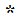
\includegraphics{fig/JamPasir/1.png}	
		\end{figure}

	\begin{center}
	\textbf{Test Case 2}\\
	\end{center}
	\textbf{Masukan}\\
	2\\
	\textbf{Keluaran}
		\begin{figure}[h!]
		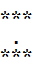
\includegraphics{fig/JamPasir/2.png}	
		\end{figure}

\pagebreak
	\begin{center}
	\textbf{Test Case 3}\\
	\end{center}
	\textbf{Masukan}\\
	3\\
	\textbf{Keluaran}\\
		\begin{figure}[h!]
		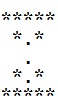
\includegraphics{fig/JamPasir/3.png}	
		\end{figure}
	\begin{center}
	\textbf{Test Case 4}\\
	\end{center}
	\textbf{Masukan}\\
	4\\
	\textbf{Keluaran}\\
		\begin{figure}[h!]
		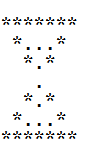
\includegraphics{fig/JamPasir/4.png}	
		\end{figure}
		\begin{center}
		\pagebreak
	\textbf{Test Case 5}\\
	\end{center}
	\textbf{Masukan}\\
	5\\
	\textbf{Keluaran}\\
		\begin{figure}[h!]
		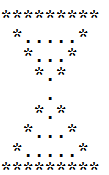
\includegraphics{fig/JamPasir/5.png}	
		\end{figure}
			
	
	Anda diminta untuk membuat sebuah fungsi untuk penyelesaian masalah ini dengan ketentuan : \\
	\begin{itemize}
		\item \textit{proc\_jamPasir(integer) : None}\\
		\item \textit{func\_jamPasir(integer) : String}\\\\
	\end{itemize}

	
	\textbf{Perhatian : Anda dianggap berhasil menjawab Permasalahan 5 jika berhasil ACCEPTED pada tiga permasalahan Problem VII-5a-Func, VII-5b-Func, VII-5c-Func untuk satu kode sumber yang sama.}
		
		
	
\end{permasalahan}




